\subsection{Generalisation}\label{sec:generalisation}
We trained DGN on standard datasets namely MNIST and CIFAR-10, under the following conditions: i) the gates are frozen $\G_t=\G_0,\forall t\geq 0$ and ii) the gating values are obtained from a ReLU network, which acts as the gating network (see \Cref{tb:dgn}). Since, the gates are frozen, the NPFs are fixed and the (stochastic) GD learns only the path values. We compare the performance of $4$ different NPFs, wherein, the gates are copied from i) from a randomly initialised ReLU network (untrained), ii) from a ReLU network trained with good dataset iii) ReLU network trained on random labels and iv) ReLU network trained on random pixels. Note that the DGN with these fixed (gates) NPFs are trained on the standard dataset with good labels. From the results in \Cref{tb:npfs}, we can conclude that NPFs are learnt during training, i.e., NPFs obtained from trained networks perform better than NPFs obtained at random initialisation.\\
%\FloatBarrier
\begin{table}[!b]
\begin{tabular}{|c|c|c|c|c|c|c|}\hline
&&&&\multicolumn{3}{c|}{NPF (trained)}\\\cline{5-7}
$(w,d)$	&Dataset		&ReLU		&NPF(Un-trained) 		&Good Label		&Random Label 	&Random Pixel\\\hline
$(128,6)$	& MNIST 		& $98.15$ 		&$96$ 		&$98.3$		&$92.6$			&$94.3$\\\hline
$(256,6)$	& MNIST 		& $98.5$ 		&$96.6$ 		&$98.4$		&$92.0$			&$81.1$\\\hline
$(256,10)$	& MNIST 		& $98.4$ 		&$96.2$ 		&$98.2$		&$72.9$			&$80.3$\\\hline
$(256,10)$	& MNIST 		& $98.4$ 		&$96.2$ 		&$98.2$		&$72.9$			&$80.3$\\\hline
\end{tabular}
\caption{Shows the training and generalisation performance of various NPFs.}
\label{tb:npfs}
\end{table}
\textbf{Relation to prior work:} As seen in \Cref{tb:npfs}, we know that, different NPFs give different generalisation performance. In this light, \Cref{th:main} complements the results by \cite{arora2019exact,cao2019generalization}, in that, one can plug-in the NPK in the place of NTK in their generalisation bounds. Further, the gap in the performance of the DNN and the NTK counterparts can be explained by the fact that the NPK is learnt during training (see \Cref{fig:gen} for more evidence).
\begin{wrapfigure}{h}{0.3\textwidth}
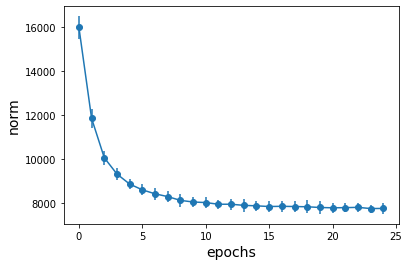
\includegraphics[scale=0.25]{figs/path-gram.png}
\caption{\label{fig:gen}$\nu_t=y^\top (\widehat{H}_t)^{-1} y$.}
\end{wrapfigure}
\textbf{NPF learning during training:} We consider ``Binary''-MNIST data set with two classes namely digits $4$ and $7$, with the labels taking values in $\{-1,+1\}$ and squared loss. We trained a standard DNN with ReLU activation ($w=100$, $d=5$). Let $\widehat{H}_t=\frac{1}{trace(H_t)}H_t$ be the normalised NPK matrix. For a subset size, $n'=200$ ($100$ examples per class) we plot $\nu_t=y^\top (\widehat{H}_t)^{-1} y$, (where $y\in\{-1,1\}^{200}$ is the labeling function), and observe that $\nu_t$ reduces as training proceeds (see \Cref{fig:gen}). \WFclear Note that, $\nu_t=\sum_{i=1}^{n'}(u_{i,t}^\top y)^2 (\hat{\rho}_{i,t})^{-1}$, where $u_{i,t}\in \R^{n'}$ are the orthonormal eigenvectors of $\widehat{H}_t$ and $\hat{\rho}_{i,t},i\in[n']$ are the corresponding eigenvalues. Since $\sum_{i=1}^{n'}\hat{\rho}_{i,t}=1$, the only way $\nu_t$ reduces is when more and more energy gets concentrated on $\hat{\rho}_{i,t}$s for which $(u_{i,t}^\top y)^2$s are also high.\\%However, in $H_t=(x^\top x)\odot \lambda_t$, only $\lambda_t$ changes with time. Thus, $\lambda_t(s,s')$ which is a measure of overlap of sub-networks active for input examples $s,s'\in[n]$, changes in a manner to reduce $\nu_t$. We can thus infer that the \emph{right} active sub-networks are learned over the course of training.\\s
\textbf{ReLU artefact:}In the case of ReLU activations (i.e., hard gates obtained for $\beta=\infty$ in \Cref{tb:dgn}), the gating values belong to $\{0,1\}$, and it follows that the activity $A_t(\cdot,\cdot)\in\{0,1\}$ and hence $\partial_{\tg} A_t(\cdot,\cdot)=0$. Consequently, there is no flow of the feature gradient in the GD update. However, since the gating parameter $\Tg$ identical with $\Theta$, (i.e., $\Tg_t=\Theta_t,\forall t$), $A_t$ changes with time due to the flow of the value gradient and NPF also changes with time. As a result, understanding feature learning in DNNs with ReLU activations is difficult, and we leave it for future work. In the next section, we study feature learning in parameterised DGNs with soft gates instead.

